\begin{frame}{Проведення експериментів}
	\manimate
	
	Для проведення експериментів існують спеціальні пакети на мові Java - CloudSim, GridSim, DARTCSIM та інші.
	
	Проблема їх усіх в тому, що вони базуються на мові Java та працюють дуже повільно у випадку великої кількості симуляцій.
	
	Тому була розроблена власне симуляційна програма.
\end{frame}

\begin{frame}{Графіки часів для різних розмірів матриць (один користувач)}
	\manimate
	
	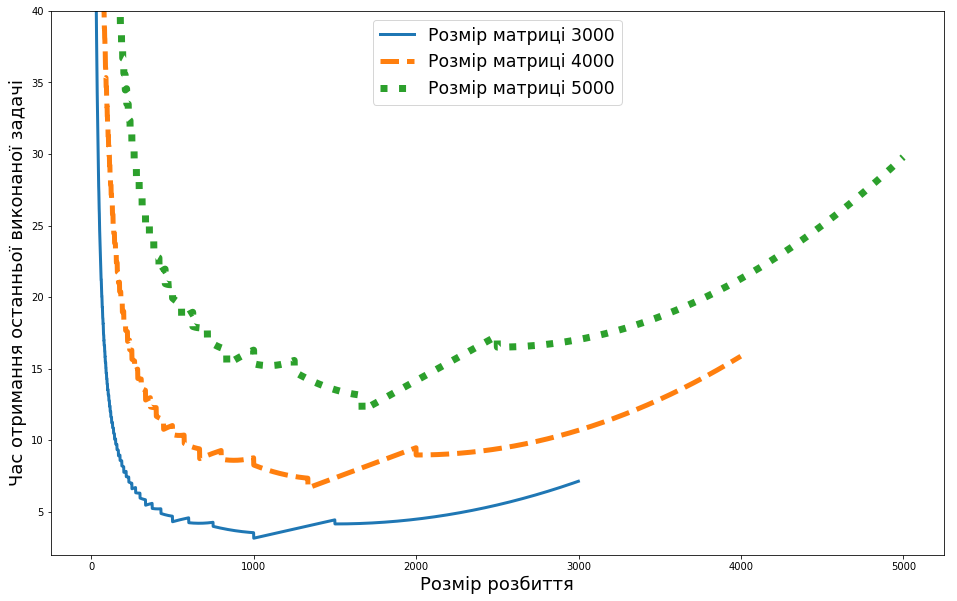
\includegraphics[width=0.8\linewidth]{im/one_user_different_N}
\end{frame}

\begin{frame}{Графіки часів для різних розмірів матриць}
	\manimate
	
	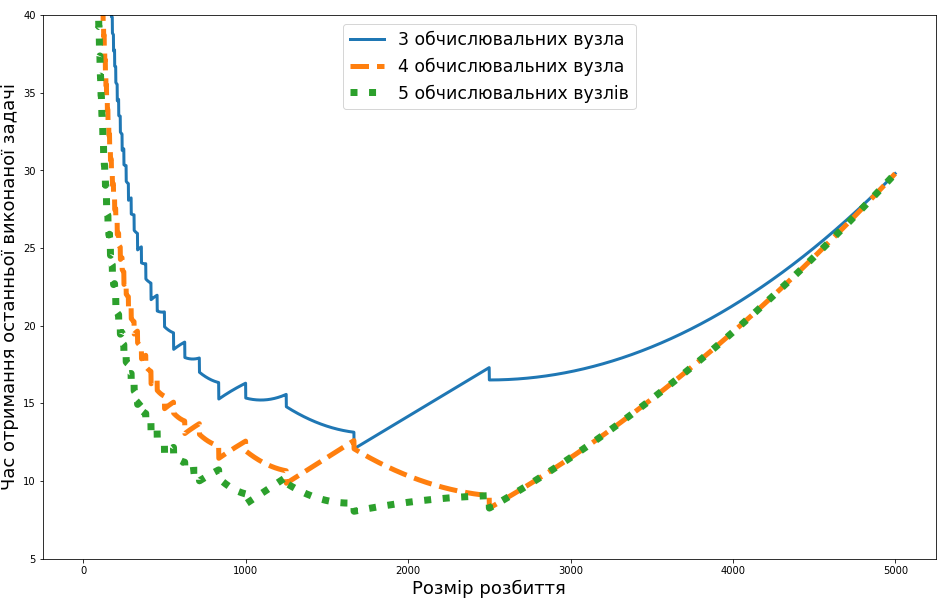
\includegraphics[width=0.9\linewidth]{im/one_user_different_proc}
\end{frame}

\begin{frame}{Графіки часів для різної кількості обчислювальних вузлів (один користувач)}
	\manimate

	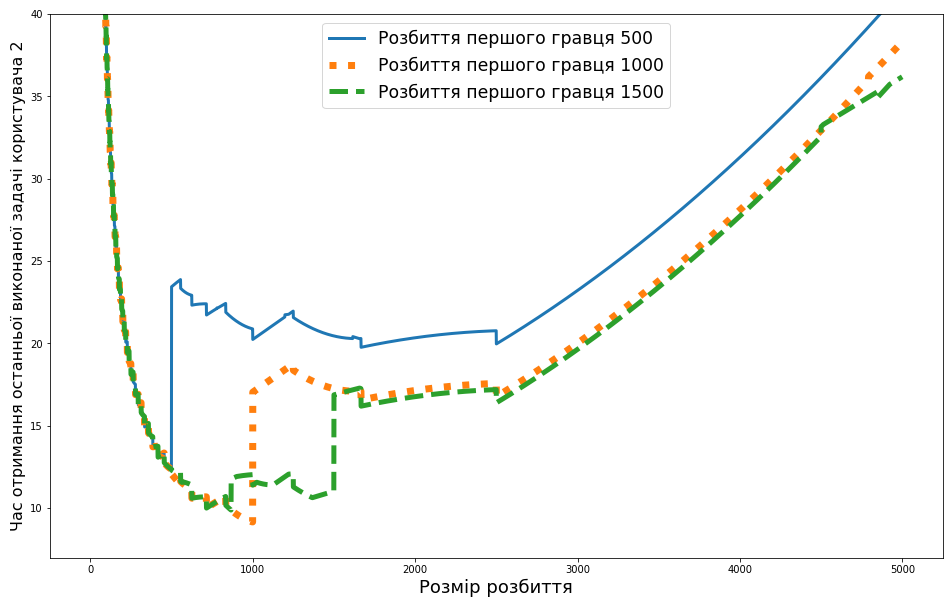
\includegraphics[width=0.7\linewidth]{im/two_users_fixed_first}
\end{frame}

\begin{frame}{Графіки часів для двох користувачів}
	\manimate

	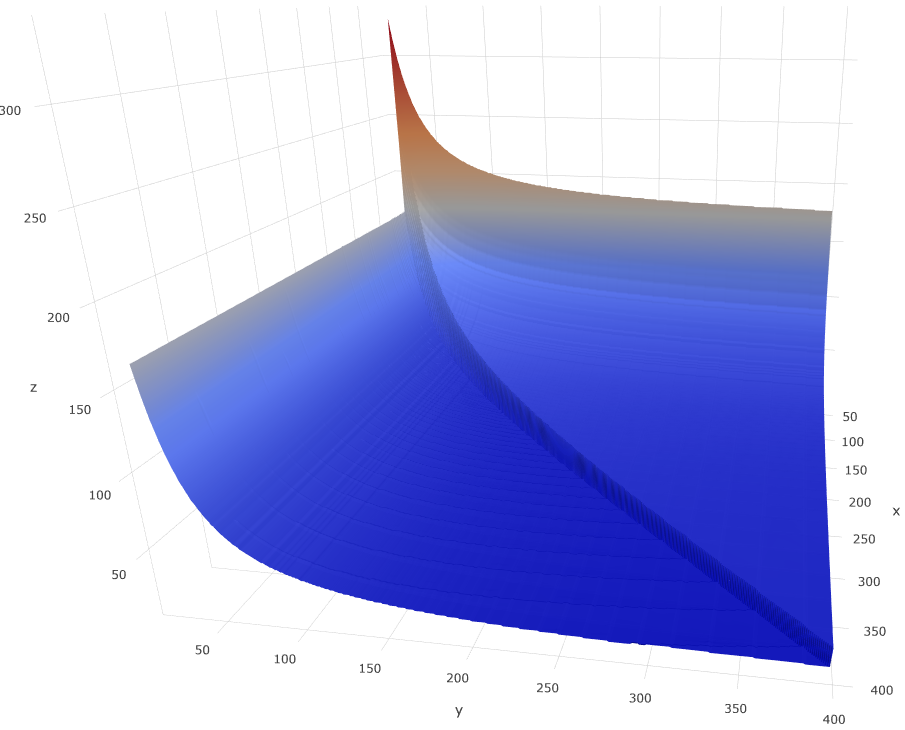
\includegraphics[width=0.6\linewidth]{im/two_users_surface_plot_20_400}
\end{frame}

\begin{frame}{Графіки часів для двох користувачів}
	\manimate
	
	\centering
	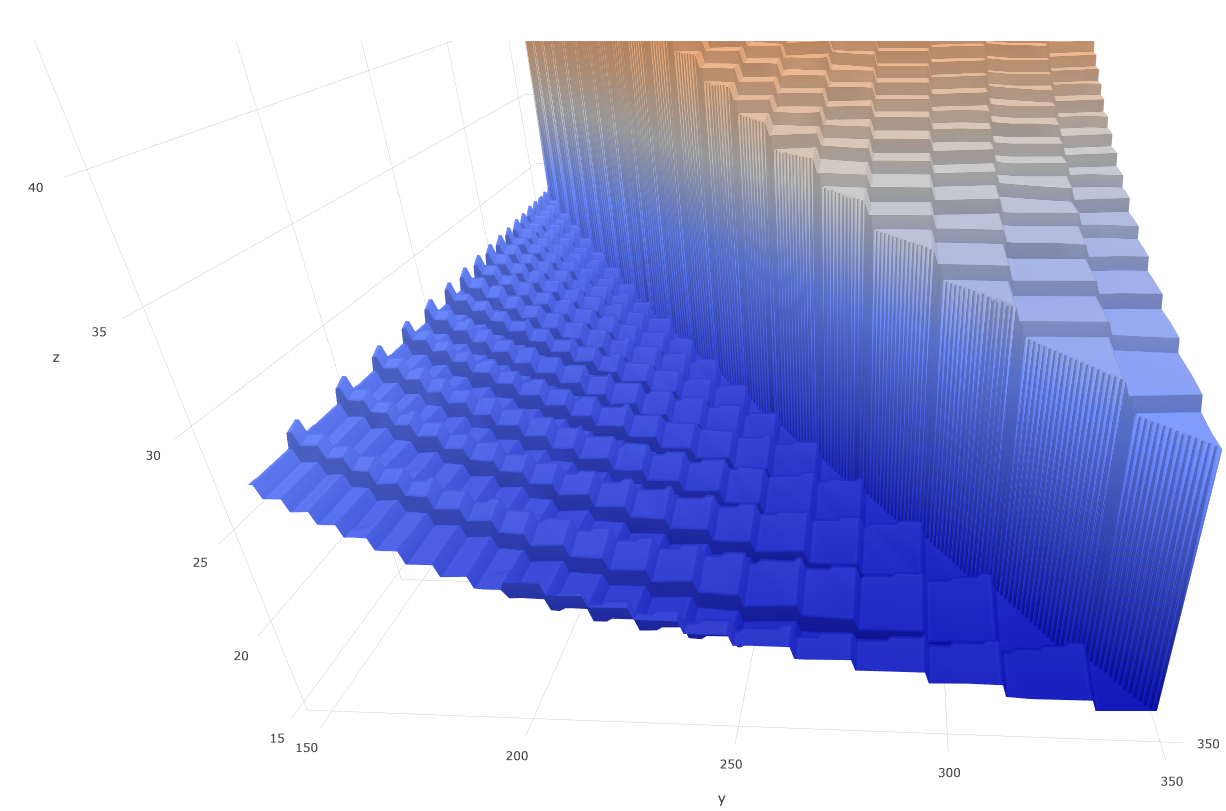
\includegraphics[width=0.4\linewidth]{im/two_users_surface_plot_150_350_bot}
	
	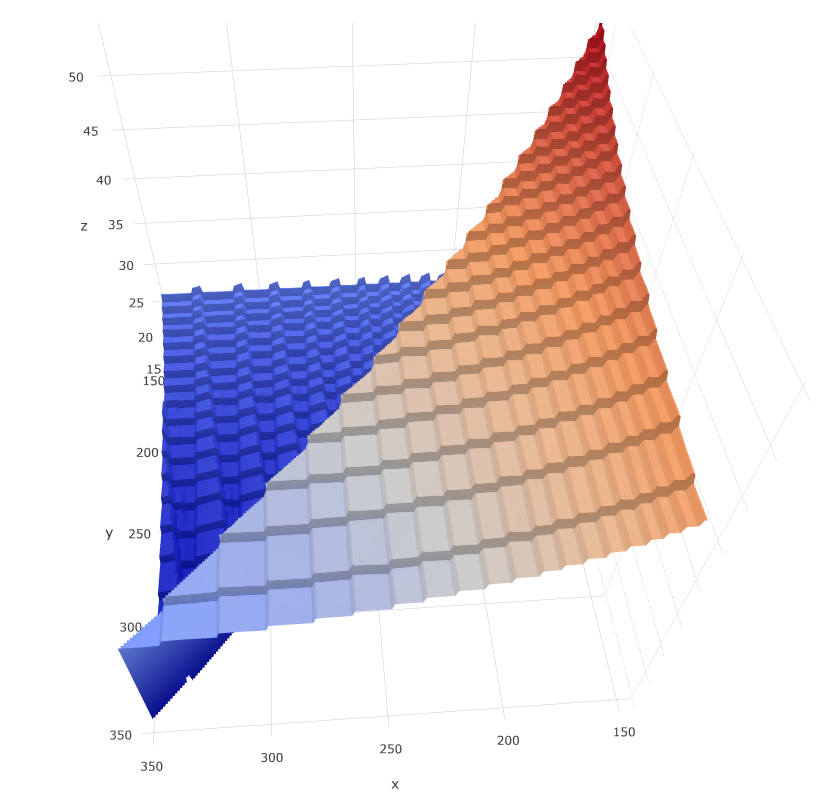
\includegraphics[width=0.4\linewidth]{im/two_users_surface_plot_150_350_top}
\end{frame}

\begin{frame}{Графіки часів для двох користувачів}
	\manimate
	
	\centering
	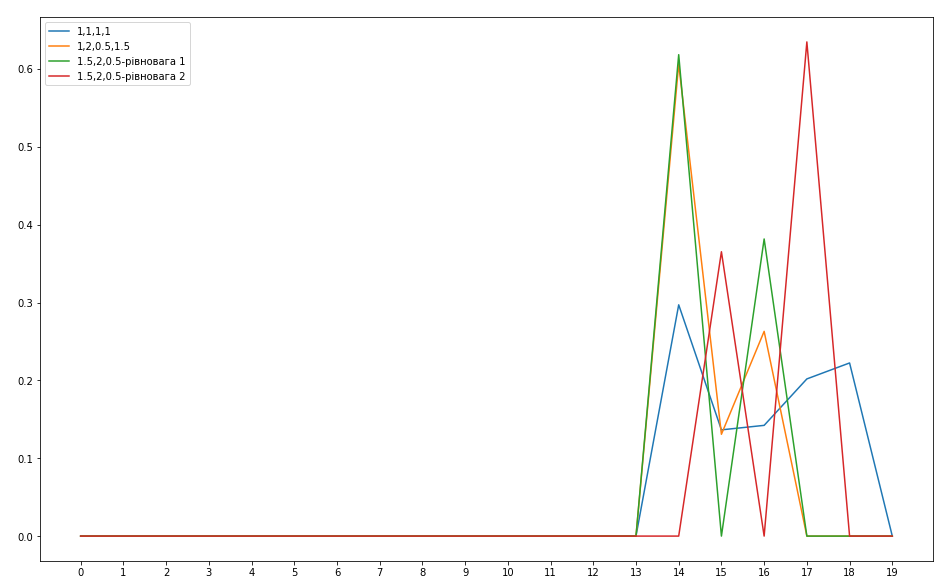
\includegraphics[width=0.6\linewidth]{im/nash_strategy_together}
\end{frame}




